% biblatex-mla.tex v1.6 2016/07/07
% Maintained at <https://github.com/jmclawson/biblatex-mla/> by James Clawson.
%
% This material is subject to the LaTeX Project Public License. Feel free to improve, redistribute, and adapt to your own ends, as allowed by that license. (See http://www.ctan.org/tex-archive/help/Catalogue/licenses.lppl.html for license details.) For inclusion in future versions, please share improvements in formatting and MLA standards compliance back to James Clawson: <biblatex-mla@konx.net>.
%
% File is in constant progress. Things are messy. Ignore platypi.

\documentclass{ltxdockit}[2011/03/25]
\usepackage{xcolor}
\usepackage{btxdockit}
\usepackage[latin9]{inputenc}
\usepackage[american]{babel}
\usepackage[strict]{csquotes}
\usepackage[style=mla,mancitepar=false]{biblatex}
\usepackage{tabularx}
\usepackage{booktabs}
\usepackage{shortvrb}
\usepackage{libertine}
\usepackage[scaled=0.8]{beramono}
\usepackage{microtype}
\usepackage{graphicx}
\usepackage{hyperref}
\hypersetup{colorlinks,% 
citecolor=black,% 
% filecolor=black,% 
% linkcolor=black,% 
% urlcolor=black}
}

\addbibresource{handbooksamples.bib}

\MakeAutoQuote{<}{>}
\MakeShortVerb{\|}

\newcommand*{\biblatexmla}{\sty{biblatex-mla}\xspace}
% \newcommand*{\biblatexmla}{Bib\latex-\textsc{mla}\xspace}
\newcommand*{\Biblatexmla}{\sty{Biblatex-mla}\xspace}
% \newcommand*{\Biblatexmla}{\biblatexmla}
\newcommand*{\biblatexmlahome}{https://github.com/jmclawson/biblatex-mla/}
\newcommand*{\biblatexmlaonctan}{http://www.ctan.org/tex-archive/help/Catalogue/entries/biblatex-mla.html}
\newcommand*{\mycode}[1]{\texttt{\textbf{#1}}}% things the user needs to type
% Use \sty{} to indicate technical things the user will never type.
\newcommand*{\mylink}[1]{$<$\url{#1}$>$}
\newcommand*{\mla}{MLA\xspace}
\newcommand*{\mycommand}[1]{\mycode{\textbackslash{}#1}}
\newcommand{\superscript}[1]{\ensuremath{^{\textrm{\tiny{#1}}}}}

\newcommand*{\biber}{\sty{biber}\xspace}
\newcommand*{\biblatex}{\sty{Biblatex}\xspace}
\newcommand*{\biblatexhome}{http://sourceforge.net/projects/biblatex/}
\newcommand*{\biblatexctan}{http://www.ctan.org/tex-archive/macros/latex/contrib/biblatex/}

\makeatletter
\newenvironment*{commandlist}
  {\list{}{%
     \setlength{\labelwidth}{\marglistwidth}%
     \setlength{\labelsep}{\marglistsep}%
     \setlength{\leftmargin}{0pt}%
     \renewcommand*{\makelabel}[1]{\hss\marglistfont##1}}%
   \def\commanditem##1{%
     \item[{\textbackslash{}##1}]%
     \ltd@pdfbookmark{##1}{##1}}}
  {\endlist}
\newenvironment*{optionslist}
  {\list{}{%
     \setlength{\labelwidth}{\marglistwidth}%
     \setlength{\labelsep}{\marglistsep}%
     \setlength{\leftmargin}{0pt}%
     \renewcommand*{\makelabel}[1]{\hss\marglistfont##1}}%
   \def\optionitem##1{%
     \item[{##1}]%
     \ltd@pdfbookmark{##1}{##1}}}
  {\endlist}
\newenvironment*{optionslistNOT}
  {\list{}{%
     \setlength{\labelwidth}{\marglistwidth}%
     \setlength{\labelsep}{\marglistsep}%
     \setlength{\leftmargin}{0pt}%
     \renewcommand*{\makelabel}[1]{\hss\marglistfont##1}}%
   \def\optionitem##1{%
     \item[{##1}]}}
  {\endlist}
\makeatother


\titlepage{%
  title={\biblatexmla},
  subtitle={\mla{} Style Using \biblatex},
  url={\biblatexmlahome},
  author={James Clawson},
  email={biblatex-mla@konx.net},
  revision={1.6},
  date={\today}}

\hypersetup{%
  pdftitle={biblatex-mla},
  pdfsubject={MLA Style Using biblatex},
  pdfauthor={James Clawson},
  pdfkeywords={mla, biblatex, bibtex, bibliography, citation}}

% colors

\definecolor{spot}{rgb}{1,0.5,0}

% tables

\newcolumntype{V}{>{\raggedright\let\\=\tabularnewline\ttfamily}p}
\newcolumntype{H}{>{\sffamily\bfseries\spotcolor}l}
\newcolumntype{P}{>{\raggedright}p{100pt}}
\newcolumntype{O}{>{\raggedright\ttfamily}p{40pt}}
\newcolumntype{S}{>{\raggedright\ttfamily}X}
\newcolumntype{N}{>{\sffamily\bfseries\spotcolor}r}
\newcolumntype{n}{>{\raggedleft\let\\\tabularnewline}p{50pt}}

\providecommand*{\numtablesetup}{\tablesetup}

\newcommand*{\sorttablesetup}{%
  \tablesetup
  \setlength{\tabcolsep}{1pt}%
  \def\new{\ensuremath\rightarrow}%
  \def\alt{\ensuremath\hookrightarrow}%
  \def\str##1{\mbox{\displayverbfont##1}}%
  \def\altstr##1{\hfill\alt\hspace{2\tabcolsep}%
    \str{##1}\hspace*{2\tabcolsep}}%
  \let\fld\bibfield}

% markup and misc

\setcounter{secnumdepth}{4}

\newrobustcmd*{\BiberOnly}{%
  \textcolor{spot}{Biber only}}
\newrobustcmd*{\BiberOnlyMark}{%
  \leavevmode\marginpar{\BiberOnly}}

\hyphenation{%
  star-red
  bib-lio-gra-phy
  white-space
  bib-latex
}

\newcommand*{\mlabibbox}[2]{\begin{center}\colorbox{#1!30}{\parbox{.9\linewidth}{#2}}\end{center}}
\newcommand*{\mlaprintbox}[2]{\begin{center}\colorbox{#1!30}{\parbox{.9\linewidth}{\begin{center}\textbf{Works Cited}\end{center}#2}}\end{center}}

\DeclareFieldFormat{braces}{\{#1\}}%
\DeclareNameAlias{default}{first-last}%
\DeclareNameAlias{author}{first-last}%
\DeclareNameAlias{editor}{first-last}%
\DeclareNameAlias{translator}{first-last}%
\DeclareNameAlias{namea}{first-last}%
\DeclareNameAlias{nameb}{first-last}%
\DeclareNameAlias{namec}{first-last}%
\DeclareListFormat{location}{%
  #1%
  \ifthenelse{\value{listcount}<\value{liststop}}
    {\addcomma\space}
    {}}%
\DeclareListFormat[article]{location}{%
  #1%
  \ifthenelse{\value{listcount}<\value{liststop}}
    {\addcomma\space}
    {}}%
\DefineBibliographyExtras{british}{%
  \protected\def\bibdatedash{$/$}
  \def\finalandcomma{}%
  \protected\def\mkbibdatelong#1#2#3{%
    \iffieldundef{#1}
      {}
      {\thefield{#1}\iffieldundef{#2}{}{-}}%
    \iffieldundef{#2}
      {}
      {\thefield{#2}\iffieldundef{#3}{}{-}}%
    \thefield{#3}}}

\renewcommand*{\multinamedelim}{\addspace\bibstring{and}\space}

\newcommand{\mlafullexample}[2]{\newline%
\mlabibbox{orange}{\begin{description}\item\mlaexample{#1}\end{description}}%
\normalfont{#2}\selectlanguage{american}%
\mlaprintbox{white}{\begin{description}\item\normalfont\fullcite{#1}\end{description}}}

\DeclareCiteCommand{\mlaexample}[\texttt]
  {\selectlanguage{british}\printtext{$@$}\printfield{entrytype}}%
  {\{\printfield{entrykey}\usebibmacro{cite:mlaexample}}%
  {}%
  {\selectlanguage{american}}
\newbibmacro*{cite:mlaexample}{%
  \setunit{\addcomma\printtext{\newline}}
  \usebibmacro{cite:mlaexample:internal}{author}%
  \usebibmacro{cite:mlaexample:internal}{authortype}%
  \usebibmacro{cite:mlaexample:internal}{bookauthor}%
  \usebibmacro{cite:mlaexample:internal}{booktitle}%
  \usebibmacro{cite:mlaexample:internal}{booksubtitle}%
  \usebibmacro{cite:mlaexample:internal}{date}%
  \usebibmacro{cite:mlaexample:internal}{edition}%
  \usebibmacro{cite:mlaexample:internal}{editor}%
  \usebibmacro{cite:mlaexample:internal}{editortype}%
  \usebibmacro{cite:mlaexample:internal}{entrysubtype}%
  \usebibmacro{cite:mlaexample:internal}{eprint}%
  \usebibmacro{cite:mlaexample:internal}{eprinttype}%
  \usebibmacro{cite:mlaexample:internal}{howpublished}%
  \usebibmacro{cite:mlaexample:internal}{institution}%
  \usebibmacro{cite:mlaexample:internal}{introduction}%
  \usebibmacro{cite:mlaexample:internal}{journaltitle}%
  \usebibmacro{cite:mlaexample:internal}{location}%
  \usebibmacro{cite:mlaexample:internal}{maintitle}%
  \usebibmacro{cite:mlaexample:internal}{mainsubtitle}%
  \usebibmacro{cite:mlaexample:internal}{nameaddon}%
  \usebibmacro{cite:mlaexample:internal}{namea}%
  \usebibmacro{cite:mlaexample:internal}{nameatype}%
  \usebibmacro{cite:mlaexample:internal}{nameb}%
  \usebibmacro{cite:mlaexample:internal}{namebtype}%
  \usebibmacro{cite:mlaexample:internal}{namec}%
  \usebibmacro{cite:mlaexample:internal}{namectype}%
  \usebibmacro{cite:mlaexample:internal}{number}%
  \usebibmacro{cite:mlaexample:internal}{options}%
  \usebibmacro{cite:mlaexample:internal}{origdate}%
  \usebibmacro{cite:mlaexample:internal}{pages}%
  \usebibmacro{cite:mlaexample:internal}{publisher}%
  \usebibmacro{cite:mlaexample:internal}{series}%
  \usebibmacro{cite:mlaexample:internal}{subtitle}%
  \usebibmacro{cite:mlaexample:internal}{title}%
  \usebibmacro{cite:mlaexample:internal}{titleaddon}%
  \usebibmacro{cite:mlaexample:internal}{translator}%
  \usebibmacro{cite:mlaexample:internal}{type}%
  \usebibmacro{cite:mlaexample:internal}{url}%
  \usebibmacro{cite:mlaexample:internal}{urldate}%
  \usebibmacro{cite:mlaexample:internal}{version}%
  \usebibmacro{cite:mlaexample:internal}{volume}%
  \setunit{\printtext{}}\printtext{\}\selectlanguage{american}%
  }%
}
\newbibmacro{cite:mlaexample:internal}[1]{%
  \ifthenelse{\equal{#1}{date}}{%
    \iffieldundef{year}{}{%
      \printtext{\indent date}%
   	  \printtext{$=$ \addspace}%
	  \printtext[braces]{\printdate}%
	}%
  }{}%
  \ifthenelse{\equal{#1}{origdate}}{%
    \iffieldundef{origyear}{}{
	  \printtext{\indent origdate}%
	  \printtext{$=$ \addspace}%
	  \printtext[braces]{\printorigdate}%
	}%
  }{}%
  \ifthenelse{\equal{#1}{urldate}}{%
    \iffieldundef{urlyear}{}{
	  \printtext{\indent urldate}%
	  \printtext{$=$ \addspace}%
	  \printtext[braces]{\printurldate}%
	}%
  }{}%
  \iffieldundef{#1}{}{%
    \printtext{\indent#1}%
	\printtext{$=$ \addspace}%
	\printfield[braces]{#1}%
  }%
  \ifnameundef{#1}{}{%
    \printtext{\indent#1}%
	\printtext{$=$ \addspace}%
	\printtext[braces]{\printnames{#1}}%
  }%
  \iflistundef{#1}{}{%
    \printtext{\indent#1}%
	\printtext{$=$ \addspace}%
	\printtext[braces]{\printlist{#1}}%
  }%
  \setunit{\addcomma\printtext{\newline}}}




\begin{document}

\printtitlepage
\tableofcontents


% \subsection{Examples} % (fold)
% \label{ssub:examples}
% \autocite{sendak63aa}

% subsection examples (end)

\section{Version Note}
This minor update addresses compatibility concerns with \biblatex. It does not reflect changes in the 8\superscript{th} edition of the \emph{MLA Handbook}, published April 2016; an upcoming version of \biblatexmla will attend to those style changes.

\section{Introduction}
\label{int}

\Biblatexmla provides support to \biblatex, \bibtex, and \latex for citations and Works Cited lists in the style established by the Modern Language Association (\mla). The style defaults to inline parenthetical citations, but it also offers support for \mla-style footnotes. For more on the commands and options for changing package defaults, see \secref{mla:subsec:commands} and \secref{mla:subsec:options}, respectively, below.

\mla style, a common standard for writers in the humanities, is outlined in the \emph{MLA Style Manual}, in its 3\superscript{rd} edition, and the \emph{MLA Handbook for Writers of Research Papers}, now in its 7\superscript{th} edition. By default, these files follow definitions for these latest editions, though they also offer the option of support for the previous style (used until 2009). \Biblatexmla also follows the logic of the \mla{} when citing similar material repeatedly, borrowing the function---but not the form---of \emph{ibid} and \emph{idem}. \Biblatexmla is compatible with \biblatex's support for \sty{hyperref} and \sty{tex2ht}, and the main word in each citation (either the author's name, the title, or the page number) serves as a link to the particular entry in the Works Cited. For anything not covered by this manual, please also see the \biblatex documentation or contact me by email.

\newpage
\section{Use}
\label{mla:sec:use}

To ensure American-style quotation marks (if that's your thing),%
%%
\footnote{Other localization files, \sty{mla-spanish.lbx}, \sty{mla-portuguese.lbx}, and \sty{mla-italian.lbx}, are also available to use \biblatexmla in languages other than English. These and other localization files are included in \biblatexmla releases, but they will not always be the latest versions available. Updated and new localization files will be uploaded to GitHub (\mylink{\biblatexmlahome}) once they are ready. There is also support for proper punctuation in non-American dialects of English. Try \mycode{british}, \mycode{canadian}, or other Babel identifiers, such as \mycode{spanish}.} %
%%
you need to call the \sty{babel} and \sty{csquotes} packages in the preamble
of your \latex document:
\begin{quote}
	\begin{verbatim}
		\usepackage[american]{babel}
		\usepackage{csquotes}
		\usepackage[style=mla]{biblatex}
		\addbibresource{<bibfile.bib>}
	\end{verbatim}	
\end{quote}
Replace <|<bibfile.bib>|> with the name of your .bib bibliography file. The style (provisionally) supports footnote citations with the \mycode{autocite=footnote} package option. Some of the other options supported by \biblatexmla include \mycode{firstlonghand}, \mycode{mladraft}, \mycode{annotation}, \mycode{noremoteinfo}, \mycode{nofullfootnote}, \mycode{publimedium}, and \mycode{guessmedium}, all discussed in \secref{mla:subsec:options}.


\subsection{Commands}
\label{mla:subsec:commands}

The standard commands for \biblatexmla generally follow those defined by \biblatex. Included below are the most typical commands. For more commands and options, reference the \biblatex manual.

\begin{commandlist}

\commanditem{autocite}
	
Insert a citation. See \tabref{use:cit:typical} for examples. For best results, use the command before punctuation like this:
\begin{quote}
	\begin{verbatim}
		\autocite{x}. 
	\end{verbatim}	
\end{quote}

\Biblatexmla defaults to parenthetical citations for \mycommand{autocite}, but a package option---\mycode{autocite=footnote}, explained below in \secref{mla:subsec:options}---changes this default behavior. In this example, |x| represents the bibkey of the particular bibliographic entry being cited. Insert page numbers and citational prenotes using square braces: 
\begin{quote}
	\begin{verbatim}
		\autocite[z][y]{x} 
	\end{verbatim}	
\end{quote}

Here, |y| is the page number, and |z| is the prenote (such as <qtd.~in>). If indicating a prenote but no page number, you must include an empty set for the page number:
\begin{quote}
	\begin{verbatim}
		\autocite[z][]{x} 
	\end{verbatim}	
\end{quote}

When citing a page number without any prenote, only one set of square brackets is needed:
\begin{quote}
	\begin{verbatim}
		\autocite[y]{x} 
	\end{verbatim}	
\end{quote}


\begin{table}
\tablesetup
\noindent\begin{tabular}{@{}V{0.33\textwidth}@{}V{0.33\textwidth}@{}p{0.3\textwidth}@{}}
\toprule
\multicolumn{1}{@{}H}{Input} &
\multicolumn{1}{@{}H}{Output} &
\multicolumn{1}{@{}H}{Comment} \\
\cmidrule(r){1-1}\cmidrule(r){2-2}\cmidrule{3-3}
\verb!\autocite[12]{morrison02aa}! & \autocite[12]{morrison02aa} & A typical citation\\
% \hline
\verb!\autocite[34]{morrison02aa}! & \autocite*[34]{morrison02aa} & Immediately subsequent citations to the same source\\% I had to star it here to show the true output that happens in a paragraph. Something about the table seems to be resetting the tracker.
% \hline
\verb!\autocite{morrison02aa}! & \autocite{morrison02aa} & Immediately subsequent citations lacking page reference \\
% \hline
\verb!\autocite[12]{frye57ab}! & \autocite[12]{frye57ab} & Citation to a text by a prolific author\\
% \hline
\verb!\autocite[34]{frye57ab}! & (34) %\autocite[34]{frye57ab} % I have to do weird things here, as the table seems to reset the tracker.
& Subsequent immediate citations to the same source\\
% \hline
\verb!\autocite[56]{frye91aa}! & \autocite*[56]{frye91aa} & Citation to new source, same author\\
% \hline
\verb!\autocite[101]{morrison02aa}! & \autocite[101]{morrison02aa} & Citation interrupting those by Frye \\
% \hline
\verb!\autocite[78]{frye91aa}! & \autocite[78]{frye91aa} & Author tracker starts over \\
\bottomrule
\end{tabular}
\caption[Typical citations]
{Syntax and output for typical citations using \biblatexmla}
\label{use:cit:typical}
\end{table}

\commanditem{autocite*}

Suppress the author's name in a citation. See \tabref{use:cit:starred} for examples. Use this starred variant of the above command when indicating the author's name in the sentence calling the citation.


\begin{table}
\tablesetup
\noindent\begin{tabular}{@{}V{0.35\textwidth}@{}V{0.3\textwidth}@{}p{0.3\textwidth}@{}}
\toprule
\multicolumn{1}{@{}H}{Input} &
\multicolumn{1}{@{}H}{Output} &
\multicolumn{1}{@{}H}{Comment} \\
\cmidrule(r){1-1}\cmidrule(r){2-2}\cmidrule{3-3}
\verb!\autocite*[102]{morrison02aa}! & \autocite*[102]{morrison02aa} & Suppressing the author's name for an entry with a single attribution to a given author prints only the page numbers\\
% \hline
\verb!\autocite*[91]{frye57ab}! & \autocite*[91]{frye57ab} & Suppressing the name of a prolific author will print enough information to avoid ambiguity\\
% \hline
\verb!\autocite*{morrison02aa}! & \autocite*{morrison02aa} & Suppressing author's name without a page number prints the title of the work\\
% \hline
\bottomrule
\end{tabular}
\caption[Suppressing the author in a citation]
{Suppressing the name of an author in citations using a starred citation command}
\label{use:cit:starred}
\end{table}

\commanditem{autocites}

Insert a citation for multiple sources at once. The respective citations will be separated by semicolons.
\begin{quote}
	\begin{verbatim}
		\autocites[z1][y1]{x1}[z2][y2]{x1}[z3][y3]{x3} 
	\end{verbatim}	
\end{quote}
The curled braces always indicate the bibkey, and the squared braces respectively belong to the curly braces that follow them.

\commanditem{mancite}

Reset only those internal trackers for \biblatexmla which shorten subsequent citations to the same work or to other works by the same author. See \tabref{use:cit:mancite} for examples. If \biblatexmla is getting so ambitious in shortening subsequent citations that it leads to ambiguity, please consider using this command before the ambiguous citation.

\begin{table}
\tablesetup
\noindent\begin{tabular}{@{}V{0.35\textwidth}@{}V{0.3\textwidth}@{}p{0.3\textwidth}@{}}
\toprule
\multicolumn{1}{@{}H}{Input} &
\multicolumn{1}{@{}H}{Output} &
\multicolumn{1}{@{}H}{Comment} \\
\cmidrule(r){1-1}\cmidrule(r){2-2}\cmidrule{3-3}
\verb!\autocite[12]{morrison02aa}! & \autocite[12]{morrison02aa} & Typical citation\\
% \hline
% \small& & \\
\verb!\mancite! \verb!   \autocite[34]{morrison02aa}! & \mancite\autocite[34]{morrison02aa} & Citation ignoring the previous citation\\
% \hline
\bottomrule
\end{tabular}
\caption[Resetting citation trackers]
{Using a command to reset trackers for shortening subsequent citation}
\label{use:cit:mancite}
\end{table}

\commanditem{citereset}

Reset all the internal trackers for \biblatexmla, including those which shorten subsequent citations to the same work or to other works by the same author and including those associated with the \mycode{firstlonghand} and \mycode{nofullfootnote} options, explained in \secref{mla:internal:firstlonghand}.

\commanditem{printbibliography}

Insert the list of Works Cited.
	
\end{commandlist}



\subsection{Package Options}
\label{mla:subsec:options}

\Biblatexmla defaults to the recommendations established by the \mla{}, but there may be times when it is appropriate to change some of these options for publication or other uses. Package options change the default functionality of \biblatexmla.

\begin{optionslist}
\optionitem{autocite=footnote}

Using \mycommand{autocite} with biblatex-mla defaults to \mla{}-preferred inline, parenthetical citations. To style citations as footnotes, set the \mycode{autocite=footnote} option in your preamble:
\begin{quote}
	\begin{verbatim}
		\usepackage[style=mla,autocite=footnote]{biblatex} 
	\end{verbatim}	
\end{quote}

\optionitem{firstlonghand}\label{mla:internal:firstlonghand}
The first citation of a source with a shorthand defined will always print a citation with author's name and, potentially, the \sty{shorttitle} field. (For more on this field, see section \secref{mla:subsec:unnusualfields}, below.) Add \mycode{firstlonghand=false} to your preamble to disable this option and print only the shorthand even on the first citation:
\begin{quote}
	\begin{verbatim}
		\usepackage[style=mla,firstlonghand=false]{biblatex} 
	\end{verbatim}	
\end{quote}

\optionitem{nofullfootnote}\label{mla:internal:nofullfootnote}
When using biblatex-mla for footnotes, the style file will provide full bibliographic detail for the first citation of every source. To turn off this option, add to your preamble \mycode{nofullfootnote}:
\begin{quote}
	\begin{verbatim}
		\usepackage[style=mla,autocite=footnote,nofullfootnote]{biblatex} 
	\end{verbatim}	
\end{quote}

\optionitem{annotation}
It is possible to print annotations to entries in the Works Cited if the \mycode{annotation} field is defined in an entry. To turn on this option, add \mycode{annotation=true} to your
preamble:
\begin{quote}
	\begin{verbatim}
		\usepackage[style=mla,annotation=true]{biblatex} 
	\end{verbatim}	
\end{quote}

\optionitem{mladraft}
When using \mla{} parenthetical citations, it is best practice to cite only when necessary to avoid ambiguity. \Biblatexmla can flag consecutive citations to the same page range, allowing you to defer citations to the end. In draft mode, \biblatexmla will place a clover ($\clubsuit$) in the margin, along with a single footnote explanation. To use the tool outside of draft mode, set the \mycode{mladraft} option in your preamble to true; similarly, to avoid seeing these clovers and the footnote in draft mode, set the option to false:
\begin{quote}
	\begin{verbatim}
		\usepackage[style=mla,mladraft=true]{biblatex}
	\end{verbatim}	
\end{quote}

\optionitem{noremoteinfo}\label{mla:internal:noremoteinfo}
Modeled after the implementation in biblatex-apa to suppress remote information in the \sty{.bib} file from being printed in the bibliography, this option affects \sty{isbn}, \sty{issn}, \sty{isrn}, \sty{doi}, and \sty{eprint} fields.
\begin{quote}
	\begin{verbatim}
		\usepackage[style=mla,noremoteinfo=true]{biblatex}
	\end{verbatim}	
\end{quote}

\optionitem{showmedium}
\Biblatexmla version 0.9 introduced support for the 3\superscript{rd} edition of the \emph{Style Manual}, requiring the publication medium of each entry to be printed in the list of Works Cited. By default, \biblatexmla will do the same, using the \sty{howpublished} field. Turn off this option---and the other new changes from the 3\superscript{rd} edition---by setting the \mycode{showmedium} option to false:
\begin{quote}
	\begin{verbatim}
		\usepackage[style=mla,showmedium=false]{biblatex}
	\end{verbatim}	
\end{quote}

\optionitem{guessmedium}
An entry with no defined \sty{howpublished} field will default either to a <Web> publication (if there's a defined \sty{url} field or \sty{eprint} field) or a <Print> publication (if there's not). To avoid \biblatexmla guessing the publication medium, thereby printing nothing when the field is undefined, deactivate the \mycode{guessmedium} option:
\begin{quote}
	\begin{verbatim}
		\usepackage[style=mla,guessmedium=false]{biblatex}
	\end{verbatim}	
\end{quote}

\optionitem{mancitepar}
Although perhaps they should, the author trackers in \biblatexmla do not by default reset with each paragraph or page. As a result, shortened citations may be unclear when much distance has passed from previous, fuller citations. To avoid this ambiguity, the \cmd{mancite} command can be called before an unclear citation. (See \tabref{use:cit:mancite} for the effects of \cmd{mancite}.) Alternatively, consider asking \biblatexmla to silently call the \cmd{mancite} command with each new paragraph by enabling the \mycode{mancitepar} package option:
\begin{quote}
	\begin{verbatim}
		\usepackage[style=mla,mancitepar=true]{biblatex}
	\end{verbatim}	
\end{quote}


\end{optionslist}

\section{Database Guide}
\label{bib}

% I lost my original documentation files, including original style files I created to maintain them, so I'm transitioning everything to Philipp Lehman's \sty{ltxdockit}. This part of the user guide, explaining how to create \sty{bibtex} entries for use with \biblatexmla, will be updated shortly. Until then, please see \S{} 4 (pages 7--20) of the previous version: \mylink{http://konx.net/biblatex-mla/biblatex-mla.pdf}.

\biblatex (and, thus, \biblatexmla) uses \bibtex-style databases to manage the citations and list of works cited. While these databases are just flat text files, there are many good programs available to help manage them. Zotero, Endnote, and other commercial programs, for example, can export as \bibtex; each of these will nevertheless export with varying degrees of success. Standalone \bibtex managers such as JabRef and BibDesk use \sty{.bib} files as their native filetype and are much more reliable for managing your list of sources. Whether exporting from a program, managing .bib files in a standalone editor, or manipulating them in a text editor, it is necessary to be familiar with fields available to \biblatexmla---especially as some of these are unique \biblatex and \biblatexmla. 

\subsection{Typical fields} % (fold)
\label{sub:typical_fields}

The best way to acquaint oneself with \biblatexmla is to explore the included \sty{.bib} files, \sty{.tex} files, and the resulting \sty{.pdf} output. Much of the the bibfile database is pretty obvious. Take a look at \tabref{fig:example-book}, for example. 
\begin{table}[tbp]
	\centering
		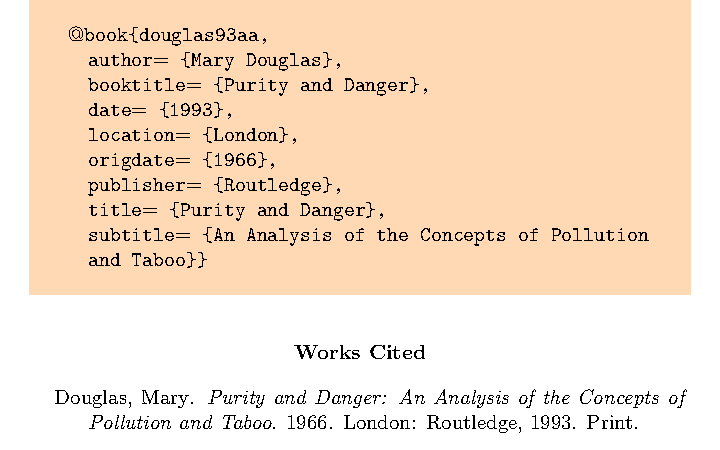
\includegraphics[width=4.8in]{example-book.pdf}
	\caption{A standard \sty{.bib} file \mycode{@book} entry and its corresponding output in the list of Works Cited, beneath.}
	\label{fig:example-book}
\end{table}

In addition to many of the standard fields one might expect to find, \biblatexmla is also capable of handling unusual fields, described below. For a fuller consideration of the fields supported by \biblatexmla, see the example files and consult the Biblatex manual.


% \mlafullexample{douglas93aa}{The above entry, found in the \sty{.bib} file, outputs to the below entry in the list of works cited:} %Below are the different \sty{@types} and the fields available to them. Keep in mind that some of the fields in the \sty{@book} and \sty{@article} types (for example, \sty{nameaddon}, \sty{origyear}, and others) are also available in others where it makes sense; I don't repeat them here to save room.

% subsection typical_fields (end)

\subsection{Unusual Fields}\label{mla:subsec:unnusualfields}
\biblatex also supports the following fields, sometimes concerned more with presentation than bibliographic merit, in all entrytypes. Define these in your \mycode{.bib} files:

\begin{optionslist}
	
	\optionitem{crossref}
	the \sty{key} of a parent source in which a shorter source is found. The \sty{crossref} field is handy to avoid spending time re-inputting similar data, but it is also useful for including \mla{}-style cross-references in the list of Works Cited. Keep in mind the problems of the \sty{crossref} field, explained in section 2.4.1 of the \biblatex manual.% In the future, \biblatexmla may provide further support for the \biblatex \sty{xref} field, making \sty{crossref} secondary in importance.
	
	\optionitem{shorttitle}
	the shortened title to be printed in citations to disambiguate among multiple titles by one author. \Biblatexmla will only print this field in citations when necessary; when this field is not defined, \biblatexmla will use the whole of the \sty{title} field.
	
	\optionitem{shorthand}
	when defined, a unique label to be printed in citations instead of the author and shorttitle. By default, \biblatexmla will only use the \sty{shorthand} label after a first citation with author (and title, if necessary). See the \mycode{firstlonghand} option on page~\pageref{mla:internal:firstlonghand} to disable this feature.
	
	\optionitem{options}
	separate the following options with a comma:
	\begin{description}
		\item[\mycode{useauthor=false}] allows the label of the entry to default to something other than the author, when the author field is defined. If the editor is defined, the label will default to that. The \mycode{useauthor} option defaults to true.
		\item[\mycode{useeditor=false}] allows the label of the entry default to something other than the editor in the case of the author field being undefined or the \mycode{useauthor} option set to false. The \mycode{useeditor} option defaults to true.
		\item[\mycode{usetranslator=true}] allows the label of the entry to inherit the name of the translator when the author and editor fields are undefined or the \mycode{useauthor} and \mycode{useeditor} options are set to false. The \mycode{usetranslator} option defaults to false.
		\item[\mycode{totalnames=true}] allows the label to include all the names in its list, rather than maxing out at three. The \mycode{totalnames} option defaults to false.
		\item[\mycode{uniquetranslator=true}] indicates that a translator of a particular \sty{@incollection} entry is unique to that work, rather than the collection at large. The \mycode{uniquetranslator} option defaults to false.
		\item[\mycode{noremoteinfo=false}] indicates that the ``remote'' information of an entry is to be printed, including the fields \sty{isbn}, \sty{issn}, \sty{isrn}, \sty{doi}, and \sty{eprint}. These fields are usually omitted. See also the global option also called \mycode{noremoteinfo}, on page~\pageref{mla:internal:noremoteinfo}, above, for defining this option on a per-document basis. The \mycode{noremoteinfo} option defaults to true.
	\end{description}	
\end{optionslist}


% \subsection{Standalone Sources}
% The following entrytypes are for long sources not part of any other publication except, potentially, multivolume sets or publishers' series.
% 
% \subsubsection*{@book}
% A book, usually with one author. \mla{}-style book entries are straightforward, and the \biblatexmla files style all the potential fields for a typical book
% 
% \begin{optionslistNOT}
% 	\optionitem{author}
% 	the author of the book
% 	
% 	\optionitem{title}
% 	book title; when using \sty{crossref}, also define \sty{booktitle} and be sure to define \sty{title} of the child entry
% 	
% 	\optionitem{subtitle}
% 	book subtitle; when using \sty{crossref}, also define \sty{booksubtitle} and be sure to define \sty{subtitle} of the child
% 	
% 	\optionitem{location}
% 	entryplace of publication
% 	
% 	\optionitem{publisher}
% 	publishing house
% 	
% 	\optionitem{year}
% 	year of publication
% \end{optionslistNOT}
% 
% Other fields might come in handy for further granularity:
% 
% \begin{optionslistNOT}
% 	\optionitem{origyear}
% 	original publication year, for reprints
% 	
% 	\optionitem{edition}
% 	edition number
% 	
% 	\optionitem{volume}
% 	volume number of book
% 	
% 	\optionitem{volumes}
% 	total number of volumes
% 	
% 	\optionitem{maintitle}
% 	title of multi-volume collection of which this book is one volume
% 	
% 	\optionitem{mainsubtitle}
% 	subtitle of the above \sty{maintitle}
% 	
% 	\optionitem{series}
% 	name of a publication series
% 	
% 	\optionitem{number}
% 	number of the above \sty{series} represented by this book
% 	
% \end{optionslistNOT}
% 
% Additionally, the style files support more name types for situations needing them:
% 
% \begin{optionslistNOT}
% 	\optionitem{editor}
% 	editor of a book	
% 	
% 	\optionitem{editortype}
% 	to indicate if the named \sty{editor} is actually an \mycode{editor} (``ed.''), a \mycode{compiler} (``comp.'') or a \mycode{compilerandeditor} (``comp. and ed.''). Default value is \mycode{editor}.
% 	
% 	\optionitem{translator}
% 	translator of a work
% 	
% 	\optionitem{introduction}
% 	author of a book's introduction
% 	
% 	\optionitem{foreword}
% 	author of a book's foreword
% 	
% 	\optionitem{afterword}
% 	author of a book's afterword
% 	
% 	\optionitem{redactor}
% 	name of redactor
% 	
% 	\optionitem{commentator}
% 	name of commentator
% 	
% 	\optionitem{annotator}
% 	name of annotator
% 	
% \end{optionslistNOT}
% 
% Finally, the style files also define the following note fields for further clarification:
% 
% \begin{optionslistNOT}
% 	\optionitem{nameaddon}
% 	pseudonym, misattribution, or other note (printed in brackets after \sty{author})
% 	
% 	\optionitem{booktitleaddon}
% 	note after the \sty{booktitle}
% 	
% 	\optionitem{maintitleaddon}
% 	note after the \sty{maintitle}
% 	
% 	\optionitem{note}
% 	miscellaneous data printed before \sty{publisher}
% 	
% 	\optionitem{addendum}
% 	miscellaneous data printed at the end of the entry
% 	
% \end{optionslistNOT}
% 
% Fields not yet supported in biblatex-mla (but which should be supported in future versions) include the following:
% 
% \begin{optionslistNOT}
% 	\optionitem{howpublished}
% 	to be used in support of the MLA-style revisions in the third edition of the \emph{MLA Style Manual} and the (upcoming) 7th edition of the \emph{MLA Handbook}; will default to ``Print''  when undefined
% 	
% 	\optionitem{origlocation}
% 	original place of publication (for reprints)
% 	
% 	\optionitem{origpublisher}
% 	original publisher (for reprints)
% 	
% 	\optionitem{origtitle}
% 	original title (for reprints)
% 	
% 	\optionitem{origlanguage}
% 	the original language of a translated, reprinted work. Biblatex-mla will not print information in this field, but if the field has information in it, it will use the phrase ``Trans. of''  before the original title, instead of ``Rept. of''.
% 	
% \end{optionslistNOT}
% 
% \subsubsection*{@booklet}
% Small pamphlet, often without an author listed. In \biblatexmla, \mycode{@booklet} is an alias for \mycode{@book} (see above), and is styled similarly.
% 
% \subsubsection*{@collection}
% A book that is a collection of self-contained essays, stories, or poems, usually with multiple unique authors and collectively edited by a single editorial body. In \biblatexmla, \mycode{@collection} is an an alias for \mycode{@book} (see above), and is styled similarly. To accurately support \mycode{@incollection} entries using \mycode{crossref}, be sure to define the following fields instead of \mycode{title} and \mycode{subtitle} in the parent \mycode{@collection} entry:
% 
% \begin{optionslistNOT}
% 	\optionitem{booktitle}
% 	the title of a book or collection
% 	
% 	\optionitem{booksubtitle}
% 	the subtitle of a book or collection	
% 	
% \end{optionslistNOT}
% 
% \subsubsection*{@periodical}
% An entire issue of a journal, usually cited by editor. \biblatexmla accepts the following fields:
% 
% \begin{optionslistNOT}
% 	\optionitem{editor}
% 	the editor or editors of an issue
% 	
% 	\optionitem{issuetitle}
% 	title of a special issue
% 	
% 	\optionitem{issuesubtitle}
% 	subtitle of a special issue
% 	
% 	\optionitem{title}
% 	title of a journal
% 	
% 	\optionitem{subtitle}
% 	subtitle of a journal
% 	
% 	\optionitem{volume}
% 	volume number of a journal
% 	
% 	\optionitem{number}
% 	issue number of a journal
% 	
% 	\optionitem{issue}
% 	season, when used in place of month (as in the ``spring'' issue of a journal)
% 	
% 	\optionitem{}
% 	
% 	\optionitem{}
% 	
% 	\optionitem{}
% 	
% \end{optionslistNOT}

\section{Meta}
\subsection{License}

\biblatexmla is copyrighted \textcopyright\ 2007--2016, by James Clawson. Permission is granted to copy, distribute, and modify this software under the terms of the \lppl, version 1.3: \mylink{http://www.ctan.org/tex-archive/macros/latex/base/lppl.txt}.

\subsection[Feedback]{Feedback}
\label{int:feb}

If you have any questions, requests, or other feedback please email me. My email address is at the top of this document. If you end up improving the code to be more accurate to the \mla{} standard, please be kind to the rest of us and share; I'm very happy to incorporate improvements! If anything works differently than you feel it ought to work, please let me know. Apart from time and my willingness to write documentation, I'm limited only by the problems of which I'm unaware.

\end{document}
